\newpage
\section{Méthodologie et planification}
\label{chap:methodologie_planification}

La planification opérationnelle est un processus essentiel pour structurer et coordonner l’exécution des tâches dans une organisation ou un projet. 
Elle repose sur des méthodes rigoureuses, des applications pratiques et des outils spécialisés pour assurer une gestion efficace des ressources, des délais et des objectifs.

Ce glossaire définit les principaux concepts liés à la planification opérationnelle et explore les méthodes, applications et outils qui permettent d’optimiser son exécution.

Dans le cadre de notre stage, nous avons appliqué une démarche méthodique et structuré notre travail pour atteindre les objectifs fixés. 
Ce chapitre détaille notre mode de travail, la planification, les outils employés ainsi que les étapes concrètes de mise en œuvre.


\subsection{Mode de travail et organisation}
Dans le besoin d’un travail optimale, le mode de travail qui s’est avéré étant la plus optimale pour notre stage fut la répartition des tâches en optant sur nos points fort. 
Cette méthode nous auras permis de renforcer nos acquis sans pour autant rester dans notre zone de confort car malgré cette méthode de travail, il y a eu derrière un grand travail d’autonomie pour approfondir la documentation ou le développement des scripts Python présent au sein du compte GitHub \textbf{Claude20022002} sur lesquelles nous devions travailler.
Notre superviseur ainsi que tous les membres du laboratoire nous ont supervisés à travers des réunions, compte rendus journalier et hebdomadaire. Pour organiser notre travail, nous avons utilisé un planning détaillé et avons tenu des comptes rendus partagés sur Github où l'on présentait nos problèmes, hypothèses et solutions.


\subsection{Planning du travail}
Afin d'assurer une progression cohérente tout au long du stage et de respecter les objectifs fixés, un planning prévisionnel a été établi dès le début du projet sous la forme d'un diagramme de Gantt. Celui-ci a permis de répartir les différentes activités sur toute la durée du stage, d'identifier les dépendances entre les tâches et de suivre l'avancement du projet.
Le déroulement du projet a été organisé en quatre grandes phases successives.
La première phase, consacrée à la \textbf{connectivité}, avait pour objectif de comprendre l'architecture matérielle et réseau du robot. Cette étape a consisté à analyser la topologie du système, identifier les différents équipements présents sur le réseau et réaliser un balayage des ports afin de découvrir les services accessibles.
La deuxième phase concernait l'\textbf{investigation du système}. Durant cette étape, plusieurs travaux de rétro-ingénierie ont été réalisés afin d'identifier les mécanismes de communication utilisés par le robot. Les services ROS ont été explorés grâce à \texttt{rosapi}, les échanges MQTT ont été analysés afin de comprendre les commandes disponibles, tandis que le fonctionnement du système de synthèse vocale a été étudié à l'aide d'ADB et d'un pont de communication Android.
La troisième phase correspond au \textbf{développement de la plateforme CYBEL}. Cette étape a constitué la partie la plus importante du projet. Elle a conduit au développement d'un SDK Python permettant de communiquer avec le robot en mode simulé ou réel, à la réalisation du backend avec FastAPI et WebSocket, à la conception de l'interface web destinée aux opérateurs ainsi qu'au développement du moteur de visite guidée, du kiosque interactif destiné aux visiteurs et de la solution de déploiement sur la tablette Android via Termux.
Enfin, la quatrième phase est dédiée à la \textbf{validation du système}. Elle comprend les essais de navigation sur le robot réel, l'ajustement des coordonnées des différents points du parcours de visite, les tests d'intégration de l'ensemble des modules développés ainsi que la rédaction du rapport de stage et la préparation de la soutenance.
La Figure~\ref{fig:gantt} présente le planning global du projet et l'enchaînement des différentes phases de réalisation.

\begin{figure}[H]
    \centering
    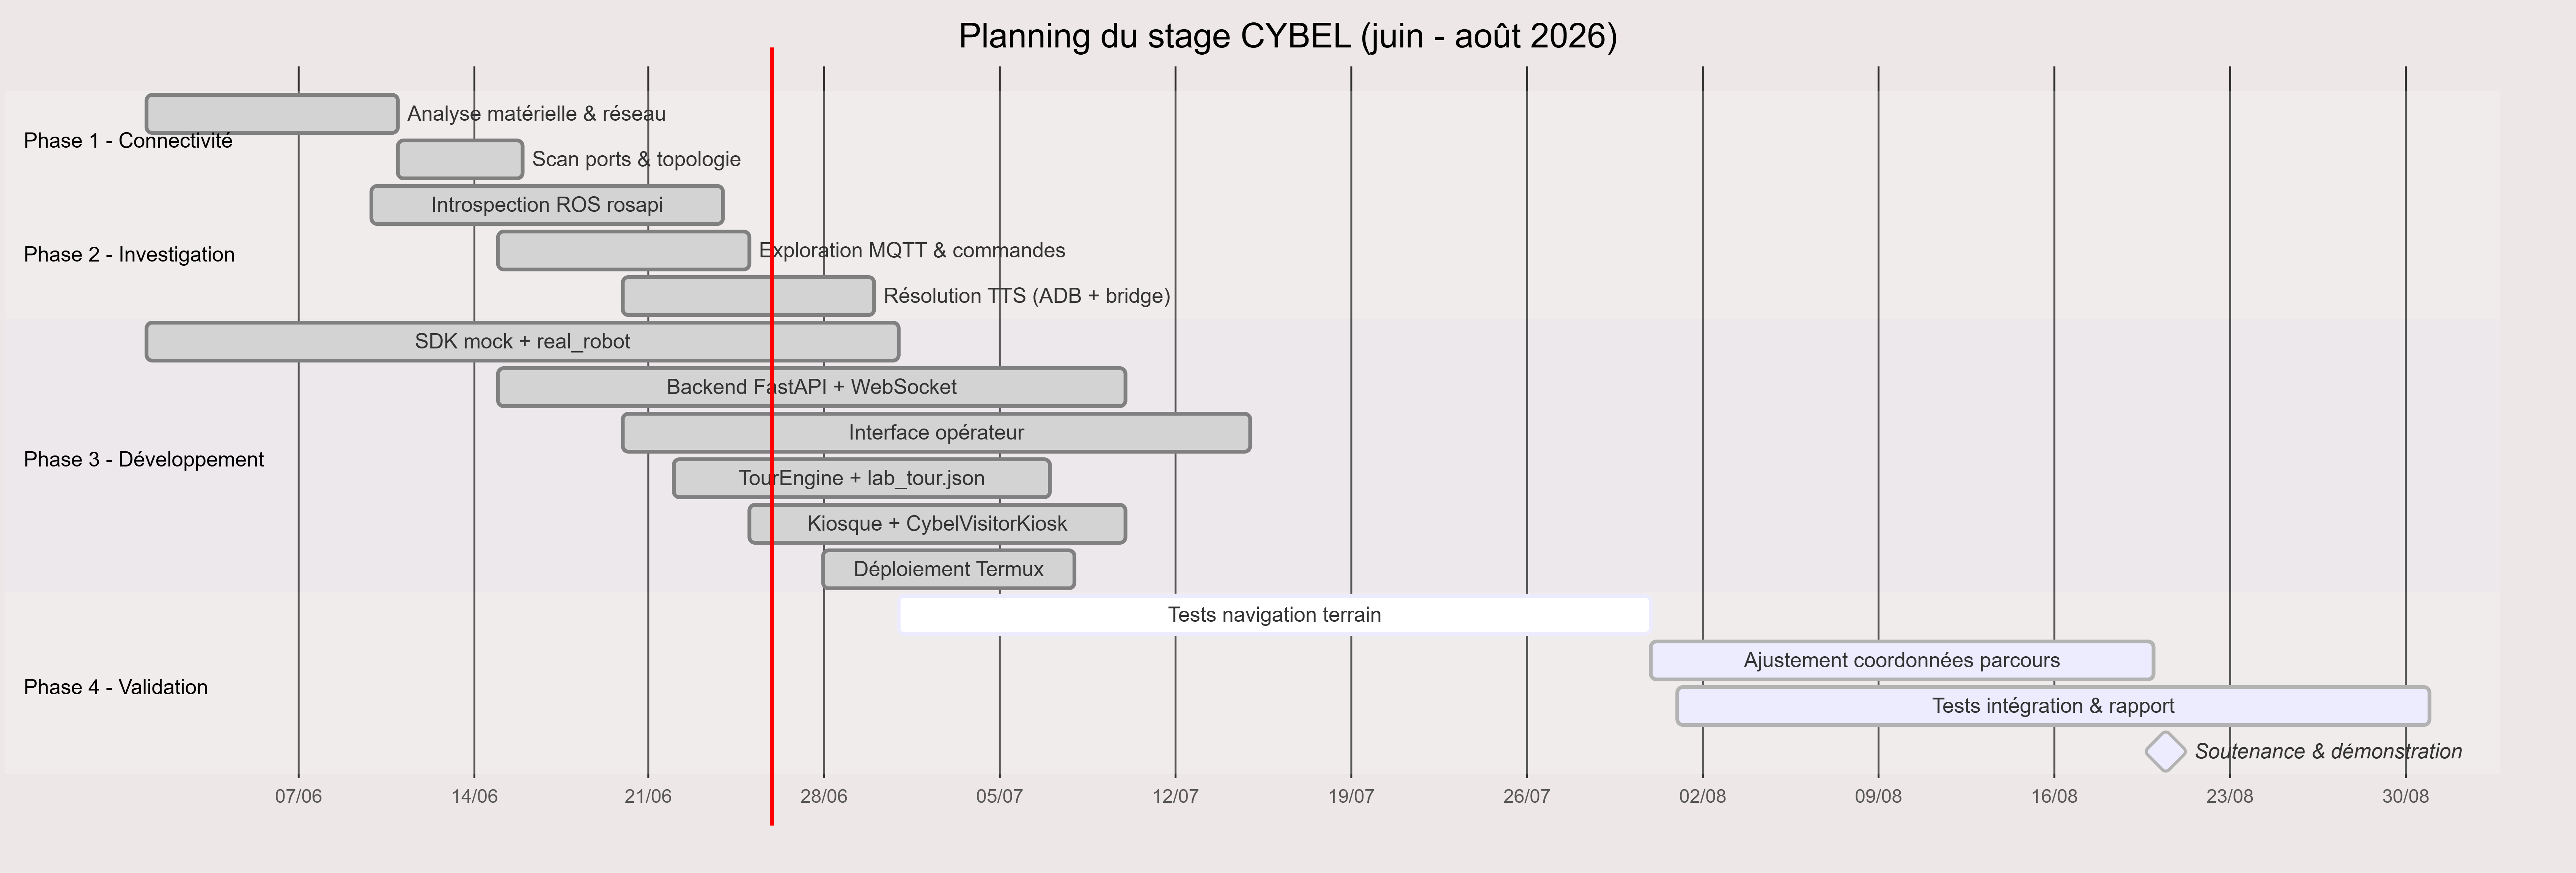
\includegraphics[width=\textwidth]{diagramme/diagramme-gantt-bg.png}
    \caption{Diagramme de Gantt du projet CYBEL}
    \label{fig:gantt}
\end{figure}

Comme le montre ce planning, plusieurs activités ont été menées en parallèle, notamment durant la phase de développement. Cette organisation a permis d'exploiter efficacement le temps disponible pendant les périodes où le robot n'était pas accessible, en poursuivant le développement de l'interface web, du backend ou des modules de simulation avant leur intégration sur le robot réel.


\subsection{Outils, Langage et Technologie utilisés}

\subsubsection{ROS}
\subsubsection{FastAPI}
\subsubsection{TypeScript}
\subsubsection{Android}
\subsubsection{ADB}
\subsubsection{ROS}

\subsection{Découverte du Robot CIOT TY1251D-03195 "CYBEL"}

\subsection{Proposition de documentation technique}

\subsection{Apports du stage}

\subsection{Difficultés rencontrées durant la phase d'investigation}

\subsection{Conclusion}